\documentclass[a4paper,10pt]{article}
\usepackage{graphicx}
\usepackage{csquotes}
\usepackage{hyperref}
\usepackage{multicol}
\usepackage{caption}
\usepackage{subcaption}
\usepackage{float}
\usepackage[a4paper,left=1.5cm,right=1.5cm,top=2cm,bottom=2cm]{geometry}
\graphicspath{ {figures/} }
\begin{document}

\begin{titlepage}
    \centering
    {\scshape\LARGE CMPT 732 Project\par}
    \vspace{1cm}
    {\Large Kyle Demeule \\ 301083503\par}
\end{titlepage}

\section*{Introduction}
Amazon is the largest online-retailer in the United States, and recently surpassed Walmart as the most valuable retailer in the U.S. by market capitalization. One of the pioneers of online-retail, Amazon had to develop techniques that would make shoppers comfortable in abandoning physical retail locations to purchase their goods online. One of these techniques was to allow anyone to review any item. Since it's inception, Amazon.com has become the largest source of internet consumer reviews. But how do customers utilize Amazon reviews? Allow me to provide a use case:

A customer knows they want a particular type of product (e.g. coffee grinder), but doesn't know anything about the best brands or models for this type of product. They go to Amazon.com, and search for \enquote{coffe grinder}. They sort the results by either \enquote{relevance} or \enquote{average customer review}, and pick an item within their price range that has a 4+ average review score with ~20+ reviews. They click that item, look at a few pictures, and then scroll down to the \enquote{Most Helpful Reviews} section. They read 1-2 of them, they're well written and positive, so they purchase the product.

This type of approach is common among Amazon customers I've talked to. It also relies heavily on the user submitted reviews, specifically their aggregate and helpfulness scores. But is it a good idea? I'll evaluate each portion.

\section*{Data Set}
For this report I will be analyzing approximately 83 million amazon reviews from May 1996 to July 2014, and metadata on approximately 9 million products. The dataset was collected by Julian McAuley, and information is available on this website (\href{http://jmcauley.ucsd.edu/data/amazon/}{link}). The reviews are in json form and compressed are about 18GB. The metadata compressed is about 3GB.

\section*{Amazon Reviews}
A user submitted review on Amazon has several components. The first is a star rating from 1 to 5. Next is a summary of the review, the main review text, and then a helpfulness score. User's can vote on a review in a yes/no fashion, stating whether they found the review helpful.

When examining user reviews it's useful to know how they are distributed. Before starting this project my expectation was something resembling a U shape, peaks at 1 and 5, and a valley at 3. The actualy distribution is a little surprising:

\begin{center}
    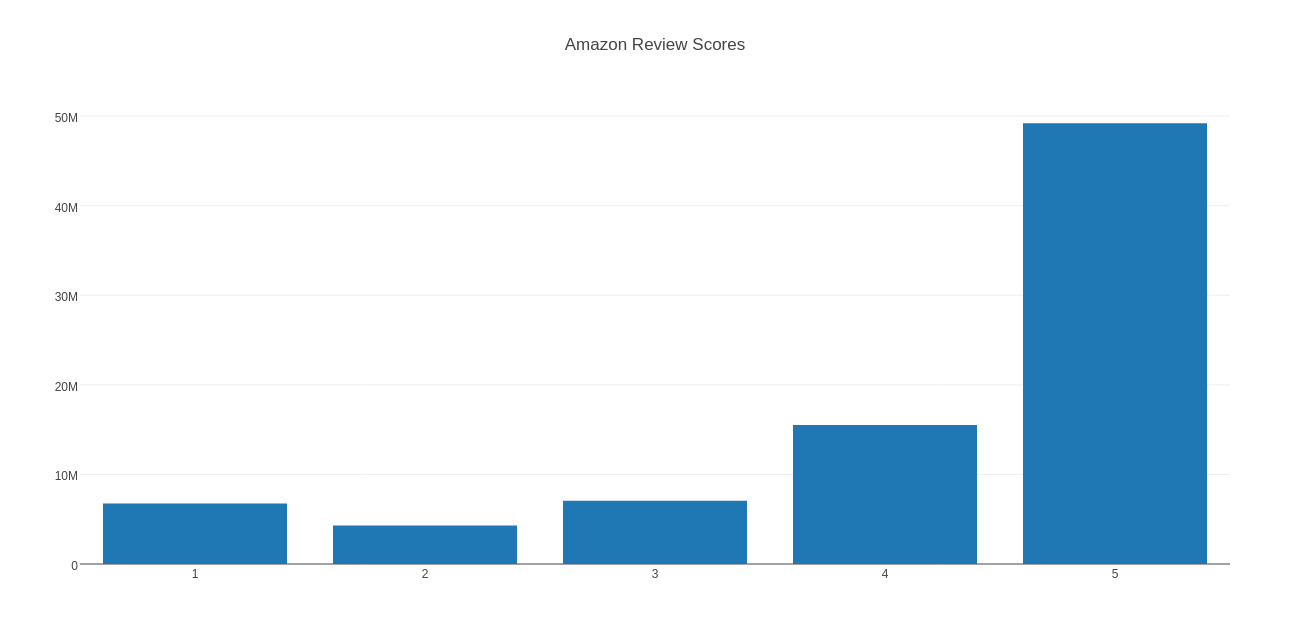
\includegraphics[scale=0.60]{score_histogram.png}
\end{center}

As we can see the reviews are intensily skewed towards 5 star reviews. In fact they make up around \textbf{42\%} of all reviews on Amazon. This distribution gives the average score of an amazon review as \textbf{4.16}, much higher than I had anticipated. However this does not mean that the average product score is 4.16, it's possible than a large number of the 5-star reviews go to the same sub-group of products, so it's worthwhile to investigate the distribution of average product review scores:

\begin{center}
    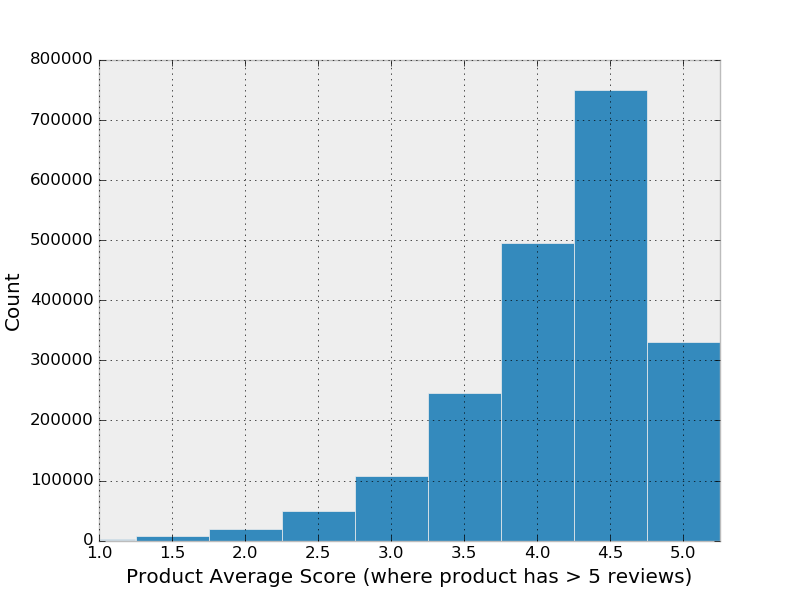
\includegraphics[scale=0.65]{starbins_gt_5.png}
\end{center}

It's worth noting that this chart only includes products with at least 5 reviews. When you include products with less you see large spikes around the X.0 and X.5 bins, which are not interesting (this is because if a product only has 1-2 reviews, it's average review score must end in X.0 or X.5, and there are a lot of products with less than 3 review scores). In the interest of finding interesing trends, and since most consumers would ignore products with little or no reviews, I will use a minimum product review condition.

Again we see a significant right skew to the distribution, with a peak at around the 4.5 mark. These bin sizes were picked for a very important reason. The Amazon UI will never actually tell you the true average score of a product, it only shows it in stars. The lowest level of granularity that the Amazon UI provides is a half star, so each of these bins corresponds to what the product would get rounded to at the center of the bin. A breakdown of the ranges:

\begin{center}
    \begin{tabular}{l l l l}
    \textbf{Range} & \textbf{Stars} & \textbf{Count} & \textbf{Percent} \\
    \hline
    1.00-1.24 & 1.0 & 1831      & 0.09\% \\
    1.25-1.74 & 1.5 & 7702      & 0.38\% \\
    1.75-2.24 & 2.0 & 19894     & 0.99\% \\
    2.25-2.74 & 2.5 & 48707     & 2.43\% \\
    2.75-3.24 & 3.0 & 107941    & 5.37\% \\
    3.25-3.74 & 3.5 & 245643    & 12.23\% \\
    3.75-4.24 & 4.0 & 495257    & 24.65\% \\
    4.25-4.74 & 4.5 & 750529    & 37.36\% \\
    4.75-5.00 & 5.0 & 331302    & 16.49\% \\
    \end{tabular}
\end{center}
What we see here is around \textbf{53\%} of products with over five reviews will show as either 4.5 or 5 stars. At least \textbf{78\%} of products with over five reviews will show as 4, 4.5, or 5 stars. This was quite shocking to me, as I used to have the impression the a product with 4.5 or 5 stars was essentially perfect, and anything with 4 or over was extremely good. There are certain types of stores that only sell products that meet a certain quality threshold, and don't carry cheaper goods (e.g. MEC), but Amazon is not one of these (their logo literally implies they carry everything from A to Z, and except in rare instances they will sell any product). The notion that nearly 4 out of 5 products on Amazon are \enquote{extremely good} is ridiculous and should be abandoned. Unless you believe that 78\% of products on amazon would meet your buying standard the star rating of a product on Amazon gives a false sense of security and should not be relied upon.


\section*{Helpfulness}
Amazon allows users to mark whether they found a review helpful or not, giving each review a helpfulness score. This score is used to pick between 1 and 8 reviews to highlight and be shown on a products page. I wondered how the distribution of reviews Amazon chose to show on a products main page compared to the total reviews for the product. Unfortunately this data was not in my original dataset, so I had to do some additional processing. I picked 2000 items at random, and retrieved the reviews Amazon displayed for them. I also retrieved each products overall count of reviews for each star rating. I compare the distribution of shown helpful reviews and total reviews here:
\begin{center}
    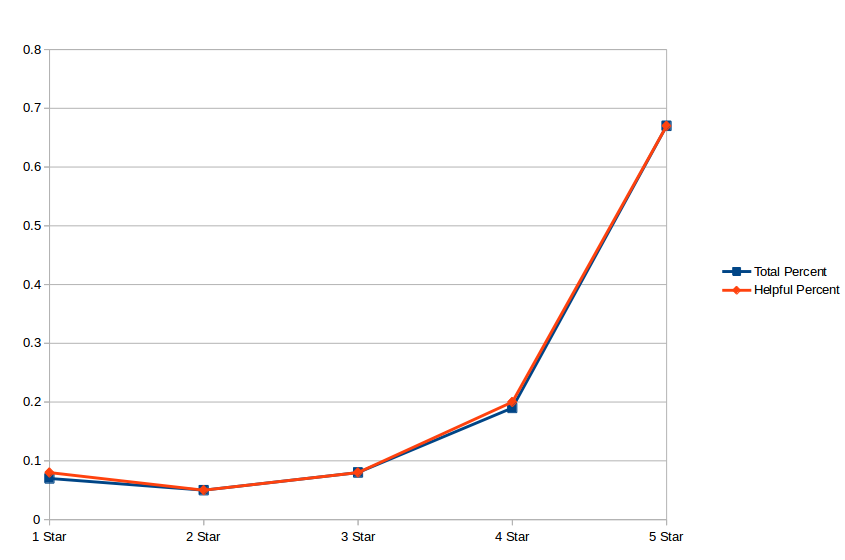
\includegraphics[scale=0.6]{helpfulness.png}
\end{center}
As we can see, they are essentially the same. This can be taken as a good thing or a bad thing. The good aspect is that the \enquote{helpful} reviews don't inflate the perception of all the reviews for the product, they are a fair representation of the rest of the reviews. The bad part is they dont inflate the reviews because the reviews were already inflated. If you randomly sampled reviews you'd see the same thing. And according to previous research, that's essentially what's being done. In 2009, Bing Liu from the University of Illinois did a study on spam in Amazon reviews. He developed a model that could predict spam to an 80\% accuracy. He analyzed the spam rating of reviews with high helpfulness scores to reviews with low helpfulness scores and found \textbf{no difference}. And this makes sense, how easy is it to mark a review as heplful? How easy would it be to game that system? (not to mention how reviews with a high number of helpful points are more visible and thus more likely to get more helpful votes)

In effect, highlighting helpful reviews is almost equivalent to highlighting random reviews, and how helpful is that?

\section*{Alternate Solution}
My original instinct was that this must be caused by spam, fraudulent reviews inflating the scores of products. But if we analyze studies done on fraudulent reviews on Amazon, this might not be the case. Recall Bing Liu's model from earlier, ~80\% accuracy at identifying spam reviews, but when they applied that to their entire data set they only found ~1\% of reviews could be considered spam. Going back to our original review score distribution diagram, nearly 50 million reviews are 5-stars. If 1\% of reviews are spam, then in the best case scenario we could remove ~800,000 reviews from the 5-star group. Unfortunately this would have little actual effect on the overall distribution, so we need a different approach.

Imagine you have a product with four reviews, and you want to see which one you trust the most. You might want to look at the history of each of the reviewers. If each one of these was one of the reviewers, who would you trust?

\begin{figure}[H]
\centering
\begin{subfigure}{.24\textwidth}
  \centering
  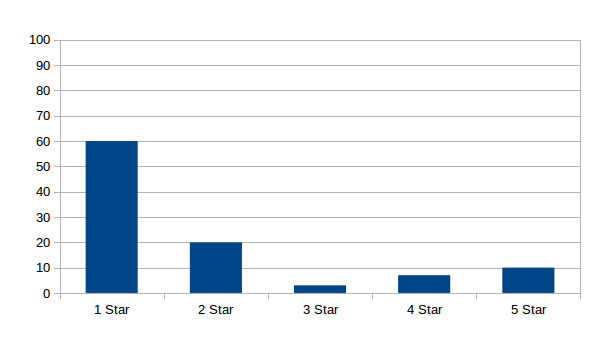
\includegraphics[width=1\linewidth]{4reviewers/neg.png}
  \label{fig:sub1}
\end{subfigure}%
\begin{subfigure}{.24\textwidth}
  \centering
  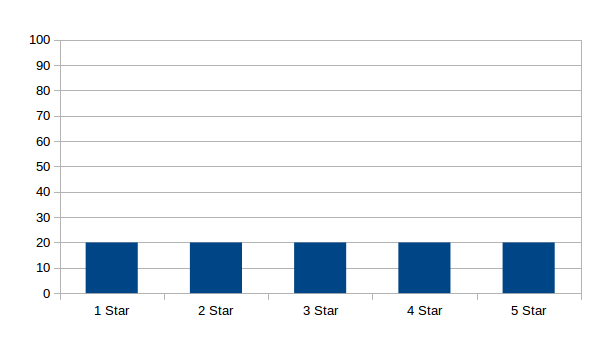
\includegraphics[width=1\linewidth]{4reviewers/uniform.png}
  \label{fig:sub2}
\end{subfigure}
\begin{subfigure}{.24\textwidth}
  \centering
  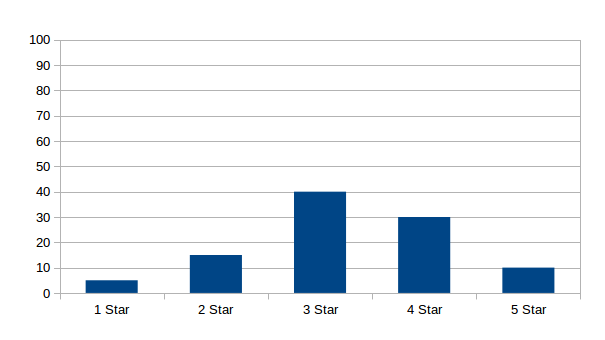
\includegraphics[width=1\linewidth]{4reviewers/norm.png}
  \label{fig:sub3}
\end{subfigure}%
\begin{subfigure}{.24\textwidth}
  \centering
  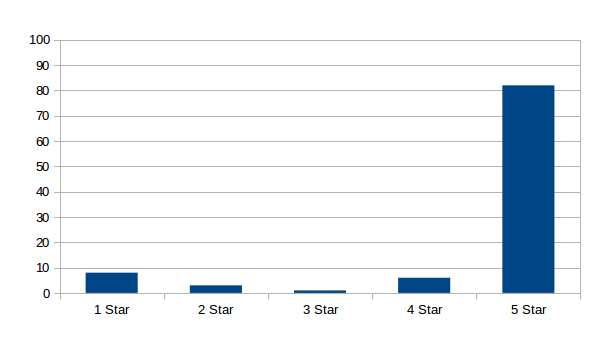
\includegraphics[width=1\linewidth]{4reviewers/pos.png}
  \label{fig:sub4}
\end{subfigure}%
\label{fig:test}
\end{figure}

Probably not the first or last one, they seem extremely biased. Maybe the second one, but the third one seems most interesting. If you're reading a 1 or 5 star review from that user, you know they mean it. And if they give a 3 star review, you're probably looking at an average product.

My idea to make Amazon reviews more useful is to create a weighted review score for each product. Give each reviewer a score based on their histogram reviews. The closer it is to my ideal history (a normal distribution in this case), the higher their score. Also favor users who have written more reviews, but with diminishing returns (for example by using a sigmoid function). Each reviewer will have a score between 0-1, use this as a weight for their reviews. If we want to pick reviews to highlight for a product, pick the ones who were written by the user with the highest rating.

Each product will now have a new aggregate score. We can compare these to the unweighted scores, and see what products increased and decreased with this new scheme. Products that decreased were likely propped up by habitual high raters (who may have been influenced to do so).

\section*{Results}
One we have new aggregate scores for each product, we can compare distribution of each with the star buckets:
\begin{center}
    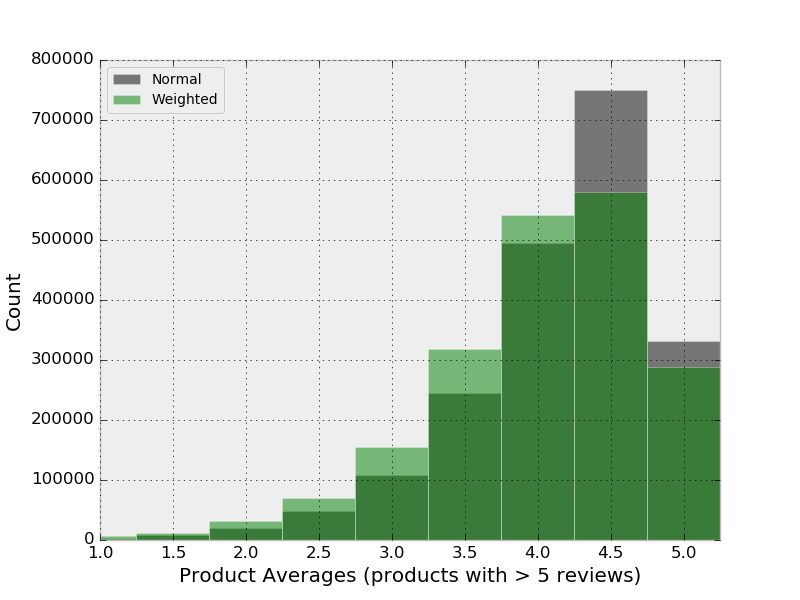
\includegraphics[scale=0.65]{normascore_vs_regular.png}
\end{center}

We can see a bit of a drift towards the left, which was the goal. There's a significant drop in 4.5 star products, a slight drop in 5 star products, and an increase in every other bucket. However we don't know if anything useful has happened yet, everything could have decreased uniformly. Let's examine how each item changed:

\begin{center}
    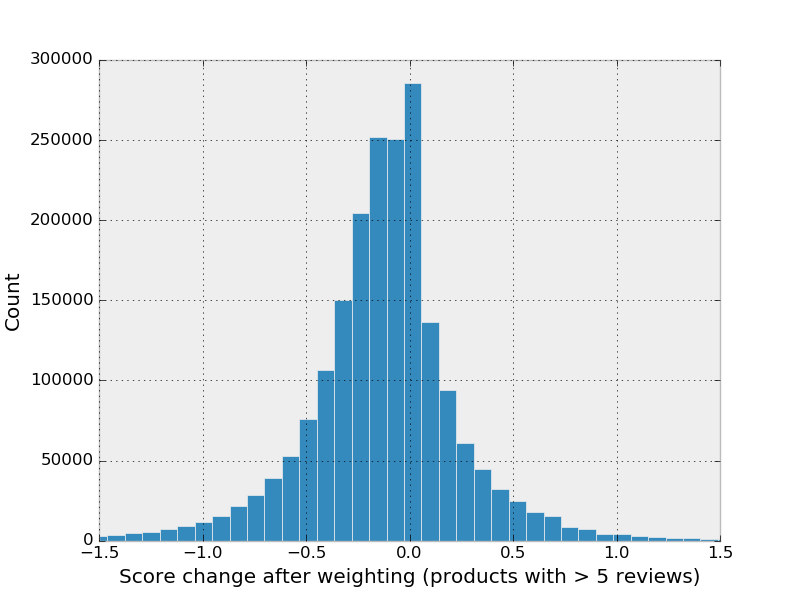
\includegraphics[scale=0.5]{normascore_changes.png}
\end{center}

Most products stayed about the same, but there's a good chunk that decreased in the -1.0 to -0.25 range, and some that even increased 1 full star. This is enough of a difference to break things down by category and brand, and see what areas benefit the most from Amazon's current biased review scores:

\begin{figure}[H]
\centering
\begin{subfigure}{.5\textwidth}
  \centering
  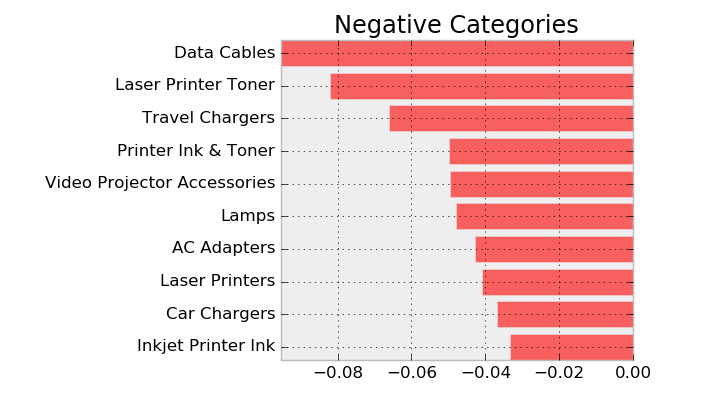
\includegraphics[width=1\linewidth]{change_by_category_neg.png}
  \label{fig:sub1}
\end{subfigure}%
\begin{subfigure}{.5\textwidth}
  \centering
  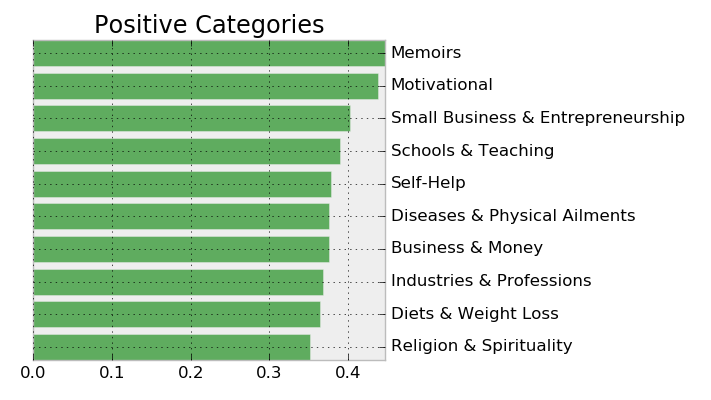
\includegraphics[width=1\linewidth]{change_by_category_pos.png}
  \label{fig:sub2}
\end{subfigure}
\label{fig:test}
\end{figure}

Only categories with at least 500 products were included in the results. The average of the difference when using the weighted scores was taken for all the products in that category. The left graph shows the 10 categories that decreased the most, and the right graph shows the categories that increased the most. Starting with those that decreased, we can see a trend in the categories. Data Cables, Travel Chargers, AC adapters, Car chargers, all in-expensive electronics. Also printers based categories make several appearances.

On the positive side we see more of a diverse set of topics. The category breakdown was actually more granular than I wanted. I was surprised to see Diet \& Weight Loss on the positive side, but when I actually looked into the products that were falling into all these categories I noticed that they were all exclusively books. This data seems to indicate that certain type of book categories might have a high number of reviews written by people who generally only write negative reviews, and that their aggregate scores are lower than they deserve.

Next we can look at how brands were affected:

\begin{figure}[H]
\centering
\begin{subfigure}{.5\textwidth}
  \centering
  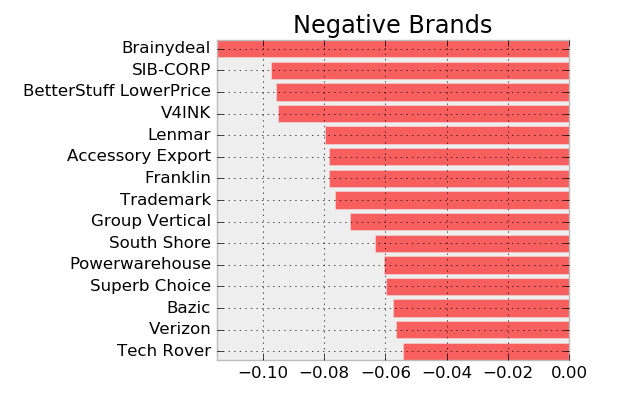
\includegraphics[width=1\linewidth]{change_by_brand_neg.png}
  \label{fig:sub1}
\end{subfigure}%
\begin{subfigure}{.5\textwidth}
  \centering
  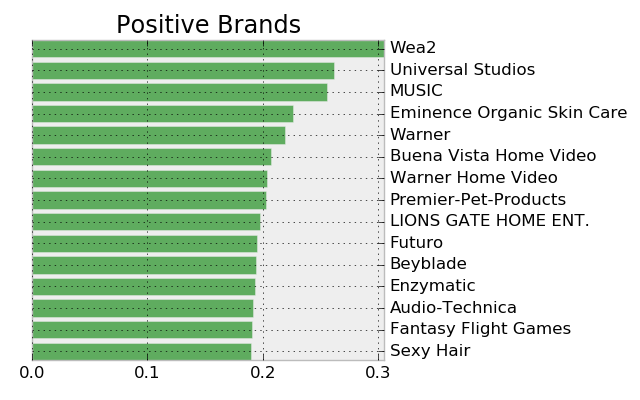
\includegraphics[width=1\linewidth]{change_by_brand_pos.png}
  \label{fig:sub2}
\end{subfigure}
\label{fig:test}
\end{figure}

There aren't many names here I recognize. What is Wea2? Searching Amazon for the term didn't reveal much. I looked at a some of the items in the dataset that had their brand as Wea2 and they were entirely music CDs. Same for the MUSIC brand. Likely this was the handle for a music distributor and many CDs got put as their brand. Something similar could be said for Warner, Universal, Lions Gate, Buena Vista(Disney), all film distribution companies that likely had many films listed under their brand. A trend here then is that multi-media like music in video has more reviews from habitually negative reviewers. Some of the more recognizable companies that are underrated are Futuro (3M subsidiary), Audio-Technica (headphones), and Enzymatic (probiotics). 

And now our worst offenders. Top of the negative list is Brainydeal, SIB-CORP, and BetterStuff LowerPrice, all of whom are low end manufacturers of cheap electronic goods. This analysis shows that it's quite likely that their products are being propped up by overly positive reviews, and should be avoided. V4INK carries print supplies, and is probably why the printer category showed up in earlier analysis. The only company from this list I had heard of before was Verizon; looking at the items they carry from the dataset it was mostly cell phone accessories like holsters and chargers. Ther overall trend here is that cheap electronics on Amazon likely have extra inflated scores relative to the rest of products.

\section*{Usage}
Originally that was all I had planned on doing for my project. But I also wanted to get some experience with new technologies, so as a last addition I wanted to store the entire dataset with my additional score information in a Cassandra database and write a web application to interact with it. The application would allow a user to search by amazon ID number and see the original and adjusted scores and histograms, as well as highlight several review. I had quasi-success with that approach, but unfortunately as of the deadline the full dataset hasn't been completely uploaded yet. The web application and structure of the cassandra are complete, and I will further discuss them in the Technology section. A running instance of the web app with dummy data (not full dataset) can be viewed at http://732.cmplx.ca/. If I'm able to get the full dataset up in time, a instance of the web app with it will be available at https://kyle732.localtunnel.me.

\section*{Technology}
All the charts were generated by me from the original data set. The dataset was converted to parquet to maintain it's compressed file size while also being easy to work with. Spark was used to calculate the aggregate scores, most were map/reduce jobs similar to what had been done in class. Calculating the alternate scores and comparisons were similar, except they involved more joins. All charts were created using matplotlib, the files to generate them can be found in the draw/ directory.

The web app to access the results is a flask application with a Cassandra database. A python cassandra driver was used to to make CQL queries against the Cassandra cluster. The queries were written manually, I didn't see the need to investigate ORM technologies for this project. All the files for the web app can be found in the web/ directory. I used a spark job to save all the information in Cassandra (cassandra\_upload.py).

The structure of the Cassandra database can be found in the CASSANDRA.md file. Cassandra is fairly interesting in that it requires you to maintain your data in a particular way if you want to make queries in a specific way. For example if you try to search based on an un-indexed query, by default Cassandra will not execute that query, displaying a warning instead. A similar situation happens when you to order the results of your queries. The general approach to order in Cassandra is that your data should be stored in the order you would want it returned in. Another aspect that is different is the primary key you use will also dictate how the records are stored in the cluster if you have multiple nodes, and in what order they are stored in (see partition key and clustering key). There's more upfront cost in designing your schema than in a typical relational database, you really need to know what type of queries you're going to be making beforehand. Also Cassandra is picky about case in column names, I had to learn this the hard way when I accidentily included mixed case column names in my Cassandra upload job (the source dataset has them in mixed case, my Cassandra database is lowercase), and upon completing a complete insert of my data into Cassandra noticed that half the columns were empty.

\section*{Project Summary}
\begin{center}
    \begin{tabular}{l l l}
    \textbf{Category} & \textbf{Score} & \textbf{Notes} \\
    \hline
    Getting the data        & 00/20 & Dataset was already compiled. \\
    ETL                     & 01/20 & Metadata file had to be processed slightly, but wasn't anything serious. \\
    Problem                 & 18/20 & \\
    Algorithmic work        & 00/20 & \\
    Bigness/parallelization & 08/20 & Dataset was not tiny. I took some shortcuts but most could scale if dataset was larger \\
    UI                      & 06/20 & There is a web front-end to access the data, it's pretty rough though. \\
    Visualization           & 12/20 & Mostly standard charts but I think I used them well and they look nice \\ 
    Technologies            & 08/20 & Worked with Cassandra for the web app \\
    \end{tabular}
\end{center}

\end{document}